%\tablesofcontent

\section{Some Results}


% ============================================
% ====== Frame : 1D Preliminary tests 1 ======
% ============================================
\subsection{1D Preliminary tests}
\begin{frame}{1D Preliminary tests}
    \begin{figure}
       \begin{tikzpicture}[scale=1.5]
      \draw[color=black,line width=2.1](0.0,0.0) -- (6.5,0);
      %\draw[color=blue, line width=10] (0,-0.02) node {$\bullet$} ;
      %\draw[color=blue, line width=10] (5,-0.02) node {$\bullet$} ;
     % \draw node[color=blue,fill,circle,minimum size=0.01](1,1) {};
      \node[anchor=south east, color=black]
      at (0,0) {};
      \node[anchor=south west, color=black]
      at (4.0,0.2) {\Large $\velocity$ ?};

      \pgfmathsetmacro{\x}{0.0}
      \draw[color=black,line width=2.1](\x,0.1) -- (\x,-0.1);

      \pgfmathsetmacro{\x}{6.5}
      \draw[color=black,line width=2.1](\x,0.1) -- (\x,-0.1);

      \pgfmathsetmacro{\x}{0.5}
      \draw[color=black,line width=1.5](\x,0.1) -- (\x,-0.1);
      \draw[color=black,line width=1.5](\x,0.1) -- (\x,-0.1);



      \pgfmathsetmacro{\x}{1.0}
      \draw[color=black,line width=1.5](\x,0.1) -- (\x,-0.1);
      \pgfmathsetmacro{\x}{1.5}

      \draw[color=black,line width=1.5](\x,0.1) -- (\x,-0.1);
      \pgfmathsetmacro{\x}{2.0}
      \draw[color=black,line width=1.5](\x,0.1) -- (\x,-0.1);
      \pgfmathsetmacro{\x}{2.5}
      \draw[color=black,line width=1.5](\x,0.1) -- (\x,-0.1);
      \pgfmathsetmacro{\x}{3.0}
      \draw[color=black,line width=1.5](\x,0.1) -- (\x,-0.1);
      \pgfmathsetmacro{\x}{3.5}
      \draw[color=black,line width=1.5](\x,0.1) -- (\x,-0.1);
      \pgfmathsetmacro{\x}{4.0}
      \draw[color=black,line width=1.5](\x,0.1) -- (\x,-0.1);
      \pgfmathsetmacro{\x}{4.5}
      \draw[color=black,line width=1.5](\x,0.1) -- (\x,-0.1);
            \pgfmathsetmacro{\x}{5.0}
      \draw[color=black,line width=1.5](\x,0.1) -- (\x,-0.1);

            \pgfmathsetmacro{\x}{5.5}
      \draw[color=black,line width=1.5](\x,0.1) -- (\x,-0.1);


            \pgfmathsetmacro{\x}{6.0}
      \draw[color=black,line width=1.5](\x,0.1) -- (\x,-0.1);

      \pgfmathsetmacro{\x}{1.5}
      \pgfmathsetmacro{\dx}{0.2}
      \pgfmathsetmacro{\y}{-0.2}
      \pgfmathsetmacro{\dy}{-0.4}
      \node (A) at (\x,\y) {}; % B = 5
      \node (B) at (\x+\dx,\y+\dy) {}; % AC = 3
      \node (C) at (\x-\dx,\y+\dy) {}; % BC = 4
      \node (receiver) at (\x,\y+\dy-0.1) {Receiver}; % BC = 4
     % \draw (A) -- (B) -- (C) -- (A);
      \begin{scope}[on background layer]
        \fill [blue] (A.center) -- (B.center) -- (C.center) -- cycle;
      \end{scope}

            \pgfmathsetmacro{\x}{0.0}
      \pgfmathsetmacro{\dx}{0.2}
      \pgfmathsetmacro{\y}{-0.2}
      \pgfmathsetmacro{\dy}{-0.4}
      \node (A) at (\x,\y) {}; % B = 5
      \node (B) at (\x+\dx,\y+\dy) {}; % AC = 3
      \node (C) at (\x-\dx,\y+\dy) {}; % BC = 4
      \node (source) at (\x,\y+\dy-0.1) {Source}; % BC = 4
      %\draw [red] (A) -- (B) -- (C) -- (A);
      \begin{scope}[on background layer]
        \fill [red] (A.center) -- (B.center) -- (C.center) -- cycle;
      \end{scope}
\end{tikzpicture}

    \end{figure}

    \begin{multicols}{2}

      \begin{center}
        Initial $\velocity$ Model
      \end{center}
      \vspace{-0.1cm}

      \setlength{\plotwidth} {4.0cm}
      \setlength{\plotheight}{3cm}
      \begin{figure}
        \centering
          \begin{tikzpicture}
      \begin{axis}[%
          width=\plotwidth, height=\plotheight,,
          at={(0,0)},scale only axis,separate axis lines,xminorticks=true,
          xlabel={Depth},
          %ylabel={$\velocity$},
          %%   ymode=log,
          yminorticks=true,
          %xmin=0.,xmax=100.,
          ymin=0.98,ymax=1.22
        ]

        %% load current data
        %% -----------------
        \addplot[color=blue!50!black,mark options={solid},
          forget plot,line width=1pt,
          mark size=2pt]
        table[x=monx,y=mony]
        {images/VP0.dat};
        %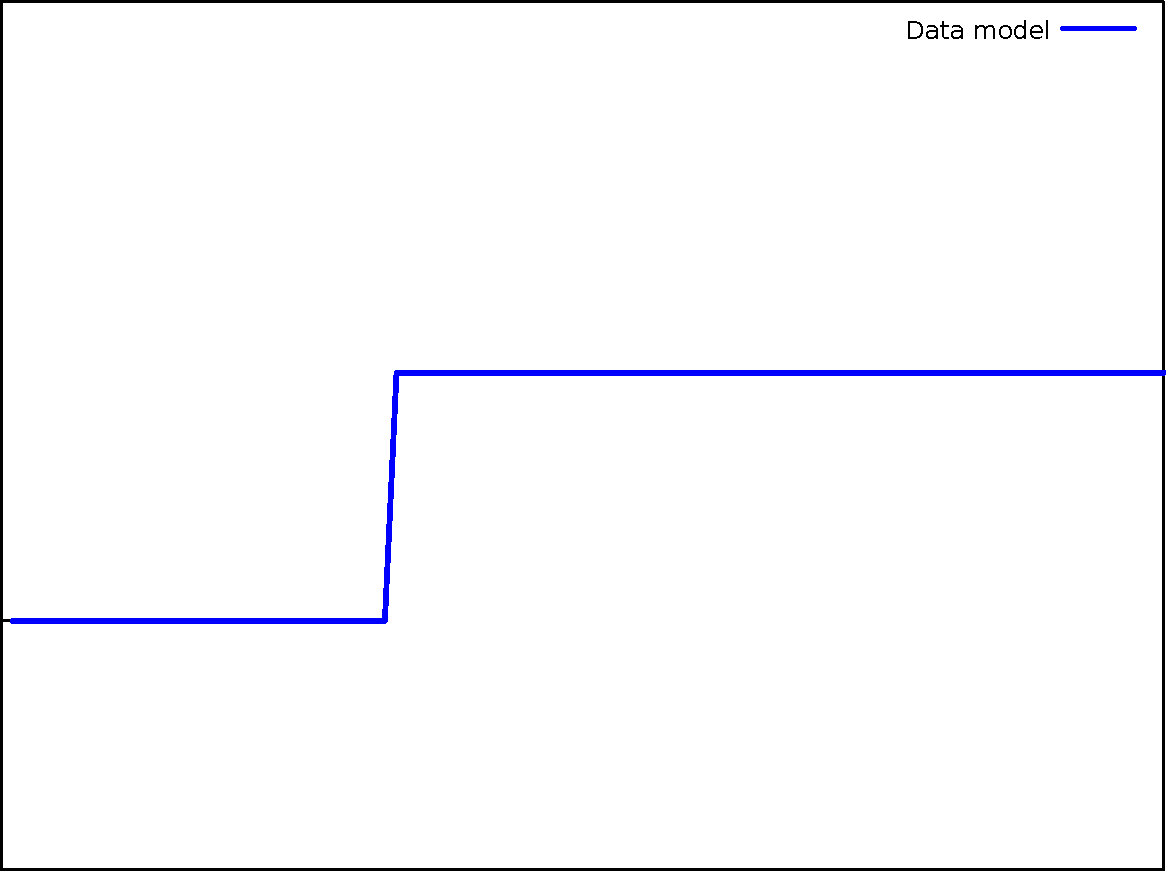
\includegraphics{images/data_bis.pdf}
      \end{axis}
      %% --------------------------------------------------------------------
          \end{tikzpicture}
          \end{figure}

      \columnbreak

      \begin{center}
        Target $\velocity$ Model
      \end{center}
      \vspace{-1.5cm}

      \begin{figure}
        \centering
          \begin{tikzpicture}
      \begin{axis}[%
          width=\plotwidth, height=\plotheight,,
          at={(0,0)},scale only axis,separate axis lines,xminorticks=true,
          xlabel={Depth},
          %ylabel={$\velocity$},
          %%   ymode=log,
          yminorticks=true,
          %%   xmin=0.,xmax=100.
        ]

        %% load current data
        %% -----------------
        \addplot[color=blue!50!black,mark options={solid},
          forget plot,line width=1pt,
          mark size=2pt]
        table[x=monx,y=mony]
        {images/VP100.dat};
      \end{axis}
      %% --------------------------------------------------------------------
          \end{tikzpicture}
          \end{figure}

      \end{multicols}

\end{frame}




% ============================================
% ====== Frame : Preliminary tests 2 =========
% ============================================

\begin{frame}{1D Preliminary tests :}
  \begin{multicols}{2}
    \normalsize
1D FWI :
\begin{itemize}
\item Lagrange / B-Bézier Operators
\item RK4 / AB3 time-schemes
\end{itemize}
\vspace{0.5cm}
\uncover<2->{
Adjoint test passed with :
\begin{itemize}
\item With a canonical space inner-product ($<u,v>_X=\sum_i u_iv_i$)
\item With a M-space inner product ($<u,v>_X^M=<Mu,v>_X$)
\end{itemize}}
\columnbreak
Gradient expression :
  \begin{equation}
     \nabla_{{\velocity}}\CF=-\int_0^{T} \int_{\Omega} \frac{2}{\density \velocity^3} \frac{\partial \contP}{\partial t}\Lbdun d\Omega dt
  \end{equation}
  \vspace{0.2cm}
  \\
  \tiny
  \uncover<2->{
\code{./run}\\
\code{----- Adjoint test -------}\\
\code{ inner product U/D   553123.57586755091    }\\
\code{ inner product G/Q   553123.57586756046    }\\
}
  %% ------------------------------------\\
  \uncover<3->{
\code{./run}\\
\code{----- Adjoint test -------}\\
\code{ inner product U/D  -75077.332007383695  }\\
\code{ inner product G/Q  -75077.332007386358  }\\
%------------------------------------\\
\code{./run}\\
\code{----- Adjoint test -------}\\
\code{ inner product U/D   125669.89223600870  }\\
\code{ inner product G/Q   125669.89223600952  }\\
}
%------------------------------------\\
\end{multicols}
\end{frame}





% ============================================
% ====== Frame : 1D Reconstruction 1 =========
% ============================================

\begin{frame}{1D Velocity Model Reconstructions}
  \setlength{\plotwidth} {10.3cm}
  \setlength{\plotheight}{6cm}
  \begin{figure}
    \centering
    \begin{tikzpicture}

      \begin{axis}[width=\plotwidth,
                   height=\plotheight,
                   xlabel={Depth},
                   ylabel={$\velocity$},
                   legend pos=south east]
        \addplot[color=red!90!black,mark options={solid},
          line width=1pt,
          mark size=2pt]
        table[x=monx,y=mony]
        {images/VP_ATD.dat};
        \addlegendentry{Adjoint Then Discretize\footnote{With Bernstein-Bézier elements}}
        \addplot[color=blue!90!black,mark options={solid},
          line width=1pt,
          mark size=2pt]
        table[x=monx,y=mony]
        {images/VP_DTA.dat};
        \addlegendentry{Discretize Then Adjoint\footnote{With canonical scalar product}}
      \end{axis}
    \end{tikzpicture}
  \end{figure}
  \begin{center}
    $\velocity$ Model at the 100th FWI iteration
  \end{center}
\end{frame}




% ============================================
% ====== Frame : 1D Reconstructions 2 ========
% ============================================
\begin{frame}{1D Velocity Model Reconstructions}

  \begin{minipage}[top]{0.5\linewidth}
    With RK4 :
  \end{minipage}
  \begin{minipage}[top]{0.4\linewidth}
    ~~~~~~~~~~~~~~~ With AB3 :
  \end{minipage}
  \begin{minipage}[top]{0.5\linewidth}
    \setlength{\plotwidth} {6.0cm}
    \setlength{\plotheight}{5cm}
      \begin{figure}
        \begin{tikzpicture}
          \begin{axis}[width=\plotwidth,
              height=\plotheight,
              ymode = log,
              ylabel near ticks, yticklabel pos=right,
              xlabel={FWI Iterations},
              legend pos=north east]
            \addplot[color=red!90!black,mark options={solid},
              line width=1pt,
              mark size=2pt]
            table[x=monx,y=mony]
            {images/run_atd_rk4_bb.txt};
            \addlegendentry{AtD}
            \addplot[color=blue!90!black,mark options={solid},
              line width=1pt,
              mark size=2pt]
            table[x=monx,y=mony]
            {images/run_dta_rk4_bb.txt};
            \addlegendentry{DtA}
          \end{axis}
        \end{tikzpicture}
      \end{figure}
    \end{minipage}\hfill
    \begin{minipage}[top]{0.5\linewidth}
      \begin{figure}
        \begin{tikzpicture}
          \setlength{\plotwidth} {6.0cm}
          \setlength{\plotheight}{5cm}
          \begin{axis}[width=\plotwidth,
              height=\plotheight,
              xlabel={FWI Iterations},
              ymode = log,
              ylabel={log(Cost Function)},
%              ylabel style={rotate=-90},
              legend pos=north east]
            \addplot[color=red!90!black,mark options={solid},
              line width=1pt,
              mark size=2pt]
            table[x=monx,y=mony]
            {images/run_atd_ab3_bb.txt};
            \addlegendentry{AtD}
            \addplot[color=blue!90!black,mark options={solid},
              line width=1pt,
              mark size=2pt]
            table[x=monx,y=mony]
            {images/run_dta_ab3_bb.txt};
            \addlegendentry{DtA}
          \end{axis}
        \end{tikzpicture}
      \end{figure}
    \end{minipage}

    \uncover<2->{
    \begin{itemize}
      \item For RK4 scheme : Similar convergency
      \item For AB3 scheme : \textcolor{red}{AtD} is slighly better than \textcolor{blue}{DtA}
      \item The slope strongly depends on the optimizer -> Impossibilty to conclude
    \end{itemize}
    }

\end{frame}





% ============================================
% ====== Frame : 2D Results Intro ============
% ============================================

\subsection{2D Time Domain FWI Results}
\begin{frame}{2D Time Domain Reconstruction}

2D FWI :
\begin{itemize}
\item Developped in Total environnement (DIP\footnote{\url{http://dip.inria.fr/}})
\item Nodal Space Operators (Lagrangian/Jacobian)
\item Modal Space Operators (Bernstein-Bézier)
\item Runge Kutta 2/4 and Adams Bashforth time-schemes
\end{itemize}
\vspace{0.5cm}
Discretize Then Adjoint strategy not implemented :
\begin{itemize}
\item Tremendous task in a complex industrial code
\end{itemize}
\end{frame}


\begin{frame}[noframenumbering]{2D Time Domain Reconstruction}

2D FWI :
\begin{itemize}
\item Developped in Total environnement (DIP\footnote{\url{http://dip.inria.fr/}})
\item Nodal Operators (Lagrangian/Jacobian)
\item Modal Operators (Bernstein-Bézier)
\item Runge Kutta 2/4 and Adams Bashforth time-schemes
\end{itemize}
\vspace{0.5cm}
 Gradient expression :
  \begin{equation}
     \nabla_{\boldsymbol{\textcolor{\mygreen}{\frac{1}{\kappa}}}}\CF=\int_0^{T} \int_{\Omega} \frac{\partial \contP}{\partial t}\Lbdun d\Omega dt \text{~~~~ with : } \boldsymbol{\textcolor{\mygreen}{\kappa}}=\density \velocity^2
  \end{equation}
   $\velocity$, $\density$ and  $\boldsymbol{\textcolor{\mygreen}{\kappa}}$  Constant per elements
\end{frame}






% ============================================
% ====== Frame : 2D Results RK/vsAB3 =========
% ============================================

\newlength{\modelwidth}
\setlength{\modelwidth}{10.8cm}
\newcommand{\modeltitle}{Initial $\velocity$ Model}

\begin{frame}{2D Time Domain FWI Reconstructions}{Time-schemes comparison}
  \vspace{-0.5cm}
  \renewcommand{\modelfile}{fig/marmousi_noise_ini}
  \begin{figure}
       \begin{tikzpicture}
\pgfmathsetmacro{\xmin} {0.}
\pgfmathsetmacro{\xmax} {12.}
\pgfmathsetmacro{\zmin} {0.}
\pgfmathsetmacro{\zmax} {2.5}

\begin{axis}[%
title={\small{\modeltitle}},
width=1.0\modelwidth,
height=0.4\modelwidth,
axis on top, separate axis lines,
xmin=\xmin, xmax=\xmax, %xlabel={x (km)},
ymin=\zmin, ymax=\zmax, ylabel={depth (km)},
yticklabels={},xticklabels={},
y dir=reverse,
colormap/paraview, colorbar,
point meta min=1.5e-3, point meta max=5.5e-3,
colorbar/width=2.5mm,
]
\addplot [forget plot] graphics [xmin=\xmin,xmax=\xmax,ymin=\zmin,ymax=\zmax] {{\modelfile}.png};
\end{axis}
\end{tikzpicture}%
 \hfill
  \end{figure}
  \vspace{-1cm}
  \renewcommand{\modeltitle}{Target $\velocity$ Model}
  \renewcommand{\modelfile}{fig/marmousi_target}
  \begin{figure}
       \begin{tikzpicture}
\pgfmathsetmacro{\xmin} {0.}
\pgfmathsetmacro{\xmax} {12.}
\pgfmathsetmacro{\zmin} {0.}
\pgfmathsetmacro{\zmax} {2.5}

\begin{axis}[%
title={\small{\modeltitle}},
width=1.0\modelwidth,
height=0.4\modelwidth,
axis on top, separate axis lines,
xmin=\xmin, xmax=\xmax, %xlabel={x (km)},
ymin=\zmin, ymax=\zmax, ylabel={depth (km)},
yticklabels={},xticklabels={},
y dir=reverse,
colormap/paraview, colorbar,
point meta min=1.5e-3, point meta max=5.5e-3,
colorbar/width=2.5mm,
]
\addplot [forget plot] graphics [xmin=\xmin,xmax=\xmax,ymin=\zmin,ymax=\zmax] {{\modelfile}.png};
\end{axis}
\end{tikzpicture}%
 \hfill
   \end{figure}
\end{frame}

\begin{frame}[noframenumbering]{2D Time Domain FWI Reconstructions}{Time-schemes comparison}
  \vspace{-0.5cm}
  \renewcommand{\modelfile}{fig/marmousi_noise_rk2}
  \renewcommand{\modeltitle}{\textbf{\textcolor{red}{RK2}} Reconstructed $\velocity$ Model (30 iterations)}
  \begin{figure}
    \begin{tikzpicture}
\pgfmathsetmacro{\xmin} {0.}
\pgfmathsetmacro{\xmax} {12.}
\pgfmathsetmacro{\zmin} {0.}
\pgfmathsetmacro{\zmax} {2.5}

\begin{axis}[%
title={\small{\modeltitle}},
width=1.0\modelwidth,
height=0.4\modelwidth,
axis on top, separate axis lines,
xmin=\xmin, xmax=\xmax, %xlabel={x (km)},
ymin=\zmin, ymax=\zmax, ylabel={depth (km)},
yticklabels={},xticklabels={},
y dir=reverse,
colormap/paraview, colorbar,
point meta min=1.5e-3, point meta max=5.5e-3,
colorbar/width=2.5mm,
]
\addplot [forget plot] graphics [xmin=\xmin,xmax=\xmax,ymin=\zmin,ymax=\zmax] {{\modelfile}.png};
\end{axis}
\end{tikzpicture}%
 \hfill
  \end{figure}
  \vspace{-1cm}
  \renewcommand{\modeltitle}{Target $\velocity$ Model}
  \renewcommand{\modelfile}{fig/marmousi_target}
  \begin{figure}
    \begin{tikzpicture}
\pgfmathsetmacro{\xmin} {0.}
\pgfmathsetmacro{\xmax} {12.}
\pgfmathsetmacro{\zmin} {0.}
\pgfmathsetmacro{\zmax} {2.5}

\begin{axis}[%
title={\small{\modeltitle}},
width=1.0\modelwidth,
height=0.4\modelwidth,
axis on top, separate axis lines,
xmin=\xmin, xmax=\xmax, %xlabel={x (km)},
ymin=\zmin, ymax=\zmax, ylabel={depth (km)},
yticklabels={},xticklabels={},
y dir=reverse,
colormap/paraview, colorbar,
point meta min=1.5e-3, point meta max=5.5e-3,
colorbar/width=2.5mm,
]
\addplot [forget plot] graphics [xmin=\xmin,xmax=\xmax,ymin=\zmin,ymax=\zmax] {{\modelfile}.png};
\end{axis}
\end{tikzpicture}%
 \hfill
  \end{figure}
\end{frame}

\begin{frame}[noframenumbering]{2D Time Domain FWI Reconstructions}{Time-schemes comparison}
  \vspace{-0.5cm}
  \renewcommand{\modelfile}{fig/marmousi_noise_rk4_2}
  \renewcommand{\modeltitle}{\textbf{\textcolor{red}{RK4}} Reconstructed $\velocity$ Model (30 iterations)}
  \begin{figure}
    \begin{tikzpicture}
\pgfmathsetmacro{\xmin} {0.}
\pgfmathsetmacro{\xmax} {12.}
\pgfmathsetmacro{\zmin} {0.}
\pgfmathsetmacro{\zmax} {2.5}

\begin{axis}[%
title={\small{\modeltitle}},
width=1.0\modelwidth,
height=0.4\modelwidth,
axis on top, separate axis lines,
xmin=\xmin, xmax=\xmax, %xlabel={x (km)},
ymin=\zmin, ymax=\zmax, ylabel={depth (km)},
yticklabels={},xticklabels={},
y dir=reverse,
colormap/paraview, colorbar,
point meta min=1.5e-3, point meta max=5.5e-3,
colorbar/width=2.5mm,
]
\addplot [forget plot] graphics [xmin=\xmin,xmax=\xmax,ymin=\zmin,ymax=\zmax] {{\modelfile}.png};
\end{axis}
\end{tikzpicture}%
 \hfill
  \end{figure}
  \vspace{-1cm}
  \renewcommand{\modeltitle}{Target $\velocity$ Model}
  \renewcommand{\modelfile}{fig/marmousi_target}
  \begin{figure}
    \begin{tikzpicture}
\pgfmathsetmacro{\xmin} {0.}
\pgfmathsetmacro{\xmax} {12.}
\pgfmathsetmacro{\zmin} {0.}
\pgfmathsetmacro{\zmax} {2.5}

\begin{axis}[%
title={\small{\modeltitle}},
width=1.0\modelwidth,
height=0.4\modelwidth,
axis on top, separate axis lines,
xmin=\xmin, xmax=\xmax, %xlabel={x (km)},
ymin=\zmin, ymax=\zmax, ylabel={depth (km)},
yticklabels={},xticklabels={},
y dir=reverse,
colormap/paraview, colorbar,
point meta min=1.5e-3, point meta max=5.5e-3,
colorbar/width=2.5mm,
]
\addplot [forget plot] graphics [xmin=\xmin,xmax=\xmax,ymin=\zmin,ymax=\zmax] {{\modelfile}.png};
\end{axis}
\end{tikzpicture}%
 \hfill
  \end{figure}
\end{frame}

\begin{frame}[noframenumbering]{2D Time Domain FWI Reconstructions}{Time-schemes comparison}
  \vspace{-0.5cm}
  \renewcommand{\modelfile}{fig/marmousi_noise_ab3}
  \renewcommand{\modeltitle}{\textbf{\textcolor{red}{AB3}} Reconstructed $\velocity$ Model (30 iterations)}
  \begin{figure}
       \begin{tikzpicture}
\pgfmathsetmacro{\xmin} {0.}
\pgfmathsetmacro{\xmax} {12.}
\pgfmathsetmacro{\zmin} {0.}
\pgfmathsetmacro{\zmax} {2.5}

\begin{axis}[%
title={\small{\modeltitle}},
width=1.0\modelwidth,
height=0.4\modelwidth,
axis on top, separate axis lines,
xmin=\xmin, xmax=\xmax, %xlabel={x (km)},
ymin=\zmin, ymax=\zmax, ylabel={depth (km)},
yticklabels={},xticklabels={},
y dir=reverse,
colormap/paraview, colorbar,
point meta min=1.5e-3, point meta max=5.5e-3,
colorbar/width=2.5mm,
]
\addplot [forget plot] graphics [xmin=\xmin,xmax=\xmax,ymin=\zmin,ymax=\zmax] {{\modelfile}.png};
\end{axis}
\end{tikzpicture}%
 \hfill
  \end{figure}
  \vspace{-1cm}
  \renewcommand{\modeltitle}{Target $\velocity$ Model}
  \renewcommand{\modelfile}{fig/marmousi_target}
  \begin{figure}
       \begin{tikzpicture}
\pgfmathsetmacro{\xmin} {0.}
\pgfmathsetmacro{\xmax} {12.}
\pgfmathsetmacro{\zmin} {0.}
\pgfmathsetmacro{\zmax} {2.5}

\begin{axis}[%
title={\small{\modeltitle}},
width=1.0\modelwidth,
height=0.4\modelwidth,
axis on top, separate axis lines,
xmin=\xmin, xmax=\xmax, %xlabel={x (km)},
ymin=\zmin, ymax=\zmax, ylabel={depth (km)},
yticklabels={},xticklabels={},
y dir=reverse,
colormap/paraview, colorbar,
point meta min=1.5e-3, point meta max=5.5e-3,
colorbar/width=2.5mm,
]
\addplot [forget plot] graphics [xmin=\xmin,xmax=\xmax,ymin=\zmin,ymax=\zmax] {{\modelfile}.png};
\end{axis}
\end{tikzpicture}%
 \hfill
   \end{figure}
\end{frame}




% ============================================
% ====== Frame : 2D Results ModalvsNodal =====
% ============================================

\begin{frame}{2D Time Domain FWI Reconstructions}{Nodal/Modal Comparison}

  \begin{multicols}{2}
    \begin{itemize}
    \item 47k P1 elements
    \item Time Scheme : AB3
    \item Constant $\density$ model ($\density=1$)
    \item 19 sources / 181 Receivers
    \item 30 iterations
    \item 120 cores
    \item Nodal computation time : 5h10
    \item Modal computation time : 7h10$^{[1]}$
    \end{itemize}
    \columnbreak

    \setlength{\plotwidth} {6.0cm}
    \setlength{\plotheight}{5cm}
    Cost function evolution :
   \begin{figure}
        \begin{tikzpicture}
          \begin{axis}[width=\plotwidth,
              height=\plotheight,
%              ymode = log,
              xlabel={FWI Iterations},
              legend pos=north east]
            \addplot[color=red!90!black,mark options={solid},
              line width=1pt,
              mark size=2pt]
            table[x=monx,y=mony]
            {fig/run_ab3_lag.txt};
            \addlegendentry{Nodal}
            \addplot[mark=*,color=blue!90!black,mark options={scale=0.7},
              line width=0pt,
              mark size=2pt]
            table[x=monx,y=mony]
            {fig/run_ab3_lag.txt};
            \addlegendentry{Modal}
          \end{axis}
        \end{tikzpicture}
      \end{figure}
  \end{multicols}

  %% pour mettre en bas et en petit
  \vfill
  \tiny
  %%%%%%%%%%%%%%%%%%%%%%%%%%%%%%%%%%
  \begin{thebibliography}{1}
  \bibitem{chan2017gpu} Chan J. and Warburton T.
    \newblock GPU-Accelerated Bernstein Bézier Discontinuous Galerkin Methods for Wave Problems
    \newblock SIAM Journal on Scientific Computing 2017
  \end{thebibliography}
\end{frame}





% ============================================
% ====== Frame : 2D Results Multiscale 1 =====
% ============================================

\subsection{2D Multiscale Reconstruction}
\begin{frame}{2D Multiscale Reconstructions}{Reconstruction with an initial smooth model}
  \vspace{-0.5cm}
  \renewcommand{\modelfile}{fig/marmousi_filter_0}
  \renewcommand{\modeltitle}{Initial $\velocity$ Model}
  \begin{figure}
       \begin{tikzpicture}
\pgfmathsetmacro{\xmin} {0.}
\pgfmathsetmacro{\xmax} {12.}
\pgfmathsetmacro{\zmin} {0.}
\pgfmathsetmacro{\zmax} {2.5}

\begin{axis}[%
title={\small{\modeltitle}},
width=1.0\modelwidth,
height=0.4\modelwidth,
axis on top, separate axis lines,
xmin=\xmin, xmax=\xmax, %xlabel={x (km)},
ymin=\zmin, ymax=\zmax, ylabel={depth (km)},
yticklabels={},xticklabels={},
y dir=reverse,
colormap/paraview, colorbar,
point meta min=1.5e-3, point meta max=5.5e-3,
colorbar/width=2.5mm,
]
\addplot [forget plot] graphics [xmin=\xmin,xmax=\xmax,ymin=\zmin,ymax=\zmax] {{\modelfile}.png};
\end{axis}
\end{tikzpicture}%
 \hfill
  \end{figure}
  \vspace{-1cm}
  \renewcommand{\modeltitle}{Target $\velocity$ Model}
  \renewcommand{\modelfile}{fig/marmousi_target}
  \begin{figure}
       \begin{tikzpicture}
\pgfmathsetmacro{\xmin} {0.}
\pgfmathsetmacro{\xmax} {12.}
\pgfmathsetmacro{\zmin} {0.}
\pgfmathsetmacro{\zmax} {2.5}

\begin{axis}[%
title={\small{\modeltitle}},
width=1.0\modelwidth,
height=0.4\modelwidth,
axis on top, separate axis lines,
xmin=\xmin, xmax=\xmax, %xlabel={x (km)},
ymin=\zmin, ymax=\zmax, ylabel={depth (km)},
yticklabels={},xticklabels={},
y dir=reverse,
colormap/paraview, colorbar,
point meta min=1.5e-3, point meta max=5.5e-3,
colorbar/width=2.5mm,
]
\addplot [forget plot] graphics [xmin=\xmin,xmax=\xmax,ymin=\zmin,ymax=\zmax] {{\modelfile}.png};
\end{axis}
\end{tikzpicture}%
 \hfill
   \end{figure}
\end{frame}

\begin{frame}[noframenumbering]{2D Multiscale Reconstructions}{Reconstruction with an initial smooth model}
  \vspace{-0.5cm}
  \renewcommand{\modelfile}{fig/marmousi_nofilter}
  \renewcommand{\modeltitle}{Reconstructed model $\velocity$ Model (30 iterations AB3)}
  \begin{figure}
       \begin{tikzpicture}
\pgfmathsetmacro{\xmin} {0.}
\pgfmathsetmacro{\xmax} {12.}
\pgfmathsetmacro{\zmin} {0.}
\pgfmathsetmacro{\zmax} {2.5}

\begin{axis}[%
title={\small{\modeltitle}},
width=1.0\modelwidth,
height=0.4\modelwidth,
axis on top, separate axis lines,
xmin=\xmin, xmax=\xmax, %xlabel={x (km)},
ymin=\zmin, ymax=\zmax, ylabel={depth (km)},
yticklabels={},xticklabels={},
y dir=reverse,
colormap/paraview, colorbar,
point meta min=1.5e-3, point meta max=5.5e-3,
colorbar/width=2.5mm,
]
\addplot [forget plot] graphics [xmin=\xmin,xmax=\xmax,ymin=\zmin,ymax=\zmax] {{\modelfile}.png};
\end{axis}
\end{tikzpicture}%
 \hfill
  \end{figure}
  \vspace{-1cm}
  \renewcommand{\modeltitle}{Target $\velocity$ Model}
  \renewcommand{\modelfile}{fig/marmousi_target}
  \begin{figure}
       \begin{tikzpicture}
\pgfmathsetmacro{\xmin} {0.}
\pgfmathsetmacro{\xmax} {12.}
\pgfmathsetmacro{\zmin} {0.}
\pgfmathsetmacro{\zmax} {2.5}

\begin{axis}[%
title={\small{\modeltitle}},
width=1.0\modelwidth,
height=0.4\modelwidth,
axis on top, separate axis lines,
xmin=\xmin, xmax=\xmax, %xlabel={x (km)},
ymin=\zmin, ymax=\zmax, ylabel={depth (km)},
yticklabels={},xticklabels={},
y dir=reverse,
colormap/paraview, colorbar,
point meta min=1.5e-3, point meta max=5.5e-3,
colorbar/width=2.5mm,
]
\addplot [forget plot] graphics [xmin=\xmin,xmax=\xmax,ymin=\zmin,ymax=\zmax] {{\modelfile}.png};
\end{axis}
\end{tikzpicture}%
 \hfill
   \end{figure}
\end{frame}





% ============================================
% ====== Frame : Multiscale principle=========
% ============================================

\begin{frame}{2D Multiscale Reconstructions}{Multiscale Principle}


  \setlength{\plotwidth} {6.0cm}
  \setlength{\plotheight}{3cm}
  \begin{figure}
    \begin{tikzpicture}
      \begin{axis}[width=\plotwidth,
          height=\plotheight,
          %              ymode = log,
          xlabel={FWI Iterations},
          ymin=-5,ymax=29
        ]
        \addplot[color=red!90!black,mark options={solid},
          line width=1pt,
          mark size=2pt]
        table[x=monx,y=mony]
        {fig/file1.txt};
      \end{axis}
    \end{tikzpicture}
  \end{figure}

  \begin{figure}
    \begin{tikzpicture}
      \begin{axis}[width=\plotwidth,
          height=\plotheight,
          %              ymode = log,
          xlabel={FWI Iterations},
        ]
        \addplot[color=red!90!black,mark options={solid},
          line width=1pt,
          mark size=2pt]
        table[x=monx,y=mony]
        {fig/file2.txt};
      \end{axis}
    \end{tikzpicture}
  \end{figure}


  \begin{figure}
    \begin{tikzpicture}
      \begin{axis}[width=\plotwidth,
          height=\plotheight,
          %              ymode = log,
          xlabel={FWI Iterations},
        ]
        \addplot[color=red!90!black,mark options={solid},
          line width=1pt,
          mark size=2pt]
        table[x=monx,y=mony]
        {fig/file3.txt};
      \end{axis}
    \end{tikzpicture}
  \end{figure}

\end{frame}






% ===============================================
% ====== Frame : 2D Multiscale reconstruction ===
% ===============================================


\begin{frame}{2D Multiscale Reconstructions}{Reconstruction with an initial smooth model}
  \vspace{-0.5cm}
  \renewcommand{\modelfile}{fig/marmousi_filter_0}
  \renewcommand{\modeltitle}{Initial $\velocity$ Model}
  \begin{figure}
       \begin{tikzpicture}
\pgfmathsetmacro{\xmin} {0.}
\pgfmathsetmacro{\xmax} {12.}
\pgfmathsetmacro{\zmin} {0.}
\pgfmathsetmacro{\zmax} {2.5}

\begin{axis}[%
title={\small{\modeltitle}},
width=1.0\modelwidth,
height=0.4\modelwidth,
axis on top, separate axis lines,
xmin=\xmin, xmax=\xmax, %xlabel={x (km)},
ymin=\zmin, ymax=\zmax, ylabel={depth (km)},
yticklabels={},xticklabels={},
y dir=reverse,
colormap/paraview, colorbar,
point meta min=1.5e-3, point meta max=5.5e-3,
colorbar/width=2.5mm,
]
\addplot [forget plot] graphics [xmin=\xmin,xmax=\xmax,ymin=\zmin,ymax=\zmax] {{\modelfile}.png};
\end{axis}
\end{tikzpicture}%
 \hfill
  \end{figure}
  \vspace{-1cm}
  \renewcommand{\modeltitle}{Target $\velocity$ Model}
  \renewcommand{\modelfile}{fig/marmousi_target}
  \begin{figure}
       \begin{tikzpicture}
\pgfmathsetmacro{\xmin} {0.}
\pgfmathsetmacro{\xmax} {12.}
\pgfmathsetmacro{\zmin} {0.}
\pgfmathsetmacro{\zmax} {2.5}

\begin{axis}[%
title={\small{\modeltitle}},
width=1.0\modelwidth,
height=0.4\modelwidth,
axis on top, separate axis lines,
xmin=\xmin, xmax=\xmax, %xlabel={x (km)},
ymin=\zmin, ymax=\zmax, ylabel={depth (km)},
yticklabels={},xticklabels={},
y dir=reverse,
colormap/paraview, colorbar,
point meta min=1.5e-3, point meta max=5.5e-3,
colorbar/width=2.5mm,
]
\addplot [forget plot] graphics [xmin=\xmin,xmax=\xmax,ymin=\zmin,ymax=\zmax] {{\modelfile}.png};
\end{axis}
\end{tikzpicture}%
 \hfill
   \end{figure}
\end{frame}

\begin{frame}[noframenumbering]{2D Multiscale Reconstructions}{Reconstruction with an initial smooth model}
  \vspace{-0.5cm}
  \renewcommand{\modelfile}{fig/marmousi_filter_1}
  \renewcommand{\modeltitle}{Reconstructed $\velocity$ Model with \textcolor{red}{1.0-2.5Hz} filter}
  \begin{figure}
       \begin{tikzpicture}
\pgfmathsetmacro{\xmin} {0.}
\pgfmathsetmacro{\xmax} {12.}
\pgfmathsetmacro{\zmin} {0.}
\pgfmathsetmacro{\zmax} {2.5}

\begin{axis}[%
title={\small{\modeltitle}},
width=1.0\modelwidth,
height=0.4\modelwidth,
axis on top, separate axis lines,
xmin=\xmin, xmax=\xmax, %xlabel={x (km)},
ymin=\zmin, ymax=\zmax, ylabel={depth (km)},
yticklabels={},xticklabels={},
y dir=reverse,
colormap/paraview, colorbar,
point meta min=1.5e-3, point meta max=5.5e-3,
colorbar/width=2.5mm,
]
\addplot [forget plot] graphics [xmin=\xmin,xmax=\xmax,ymin=\zmin,ymax=\zmax] {{\modelfile}.png};
\end{axis}
\end{tikzpicture}%
 \hfill
  \end{figure}
  \vspace{-1cm}
  \renewcommand{\modeltitle}{Target $\velocity$ Model}
  \renewcommand{\modelfile}{fig/marmousi_target}
  \begin{figure}
       \begin{tikzpicture}
\pgfmathsetmacro{\xmin} {0.}
\pgfmathsetmacro{\xmax} {12.}
\pgfmathsetmacro{\zmin} {0.}
\pgfmathsetmacro{\zmax} {2.5}

\begin{axis}[%
title={\small{\modeltitle}},
width=1.0\modelwidth,
height=0.4\modelwidth,
axis on top, separate axis lines,
xmin=\xmin, xmax=\xmax, %xlabel={x (km)},
ymin=\zmin, ymax=\zmax, ylabel={depth (km)},
yticklabels={},xticklabels={},
y dir=reverse,
colormap/paraview, colorbar,
point meta min=1.5e-3, point meta max=5.5e-3,
colorbar/width=2.5mm,
]
\addplot [forget plot] graphics [xmin=\xmin,xmax=\xmax,ymin=\zmin,ymax=\zmax] {{\modelfile}.png};
\end{axis}
\end{tikzpicture}%
 \hfill
   \end{figure}
\end{frame}

\begin{frame}[noframenumbering]{2D Multiscale Reconstructions}{Reconstruction with an initial smooth model}
  \vspace{-0.5cm}
  \renewcommand{\modelfile}{fig/marmousi_filter_2}
  \renewcommand{\modeltitle}{Reconstructed $\velocity$ Model with \textcolor{red}{1.0-7.5Hz} filter}
  \begin{figure}
       \begin{tikzpicture}
\pgfmathsetmacro{\xmin} {0.}
\pgfmathsetmacro{\xmax} {12.}
\pgfmathsetmacro{\zmin} {0.}
\pgfmathsetmacro{\zmax} {2.5}

\begin{axis}[%
title={\small{\modeltitle}},
width=1.0\modelwidth,
height=0.4\modelwidth,
axis on top, separate axis lines,
xmin=\xmin, xmax=\xmax, %xlabel={x (km)},
ymin=\zmin, ymax=\zmax, ylabel={depth (km)},
yticklabels={},xticklabels={},
y dir=reverse,
colormap/paraview, colorbar,
point meta min=1.5e-3, point meta max=5.5e-3,
colorbar/width=2.5mm,
]
\addplot [forget plot] graphics [xmin=\xmin,xmax=\xmax,ymin=\zmin,ymax=\zmax] {{\modelfile}.png};
\end{axis}
\end{tikzpicture}%
 \hfill
  \end{figure}
  \vspace{-1cm}
  \renewcommand{\modeltitle}{Target $\velocity$ Model}
  \renewcommand{\modelfile}{fig/marmousi_target}
  \begin{figure}
       \begin{tikzpicture}
\pgfmathsetmacro{\xmin} {0.}
\pgfmathsetmacro{\xmax} {12.}
\pgfmathsetmacro{\zmin} {0.}
\pgfmathsetmacro{\zmax} {2.5}

\begin{axis}[%
title={\small{\modeltitle}},
width=1.0\modelwidth,
height=0.4\modelwidth,
axis on top, separate axis lines,
xmin=\xmin, xmax=\xmax, %xlabel={x (km)},
ymin=\zmin, ymax=\zmax, ylabel={depth (km)},
yticklabels={},xticklabels={},
y dir=reverse,
colormap/paraview, colorbar,
point meta min=1.5e-3, point meta max=5.5e-3,
colorbar/width=2.5mm,
]
\addplot [forget plot] graphics [xmin=\xmin,xmax=\xmax,ymin=\zmin,ymax=\zmax] {{\modelfile}.png};
\end{axis}
\end{tikzpicture}%
 \hfill
   \end{figure}
\end{frame}

\begin{frame}[noframenumbering]{2D Multiscale Reconstructions}{Reconstruction with an initial smooth model}
  \vspace{-0.5cm}
  \renewcommand{\modelfile}{fig/marmousi_filter_3}
  \renewcommand{\modeltitle}{Reconstructed $\velocity$ Model with \textcolor{red}{1.0-10Hz} filter}
  \begin{figure}
       \begin{tikzpicture}
\pgfmathsetmacro{\xmin} {0.}
\pgfmathsetmacro{\xmax} {12.}
\pgfmathsetmacro{\zmin} {0.}
\pgfmathsetmacro{\zmax} {2.5}

\begin{axis}[%
title={\small{\modeltitle}},
width=1.0\modelwidth,
height=0.4\modelwidth,
axis on top, separate axis lines,
xmin=\xmin, xmax=\xmax, %xlabel={x (km)},
ymin=\zmin, ymax=\zmax, ylabel={depth (km)},
yticklabels={},xticklabels={},
y dir=reverse,
colormap/paraview, colorbar,
point meta min=1.5e-3, point meta max=5.5e-3,
colorbar/width=2.5mm,
]
\addplot [forget plot] graphics [xmin=\xmin,xmax=\xmax,ymin=\zmin,ymax=\zmax] {{\modelfile}.png};
\end{axis}
\end{tikzpicture}%
 \hfill
  \end{figure}
  \vspace{-1cm}
  \renewcommand{\modeltitle}{Target $\velocity$ Model}
  \renewcommand{\modelfile}{fig/marmousi_target}
  \begin{figure}
       \begin{tikzpicture}
\pgfmathsetmacro{\xmin} {0.}
\pgfmathsetmacro{\xmax} {12.}
\pgfmathsetmacro{\zmin} {0.}
\pgfmathsetmacro{\zmax} {2.5}

\begin{axis}[%
title={\small{\modeltitle}},
width=1.0\modelwidth,
height=0.4\modelwidth,
axis on top, separate axis lines,
xmin=\xmin, xmax=\xmax, %xlabel={x (km)},
ymin=\zmin, ymax=\zmax, ylabel={depth (km)},
yticklabels={},xticklabels={},
y dir=reverse,
colormap/paraview, colorbar,
point meta min=1.5e-3, point meta max=5.5e-3,
colorbar/width=2.5mm,
]
\addplot [forget plot] graphics [xmin=\xmin,xmax=\xmax,ymin=\zmin,ymax=\zmax] {{\modelfile}.png};
\end{axis}
\end{tikzpicture}%
 \hfill
   \end{figure}
\end{frame}

\begin{frame}[noframenumbering]{2D Multiscale Reconstructions}{Reconstruction with an initial smooth model}
  \vspace{-0.5cm}
  \renewcommand{\modelfile}{fig/marmousi_filter_5}
  \renewcommand{\modeltitle}{Reconstructed $\velocity$ Model with \textcolor{red}{1.0-15Hz} filter}
  \begin{figure}
       \begin{tikzpicture}
\pgfmathsetmacro{\xmin} {0.}
\pgfmathsetmacro{\xmax} {12.}
\pgfmathsetmacro{\zmin} {0.}
\pgfmathsetmacro{\zmax} {2.5}

\begin{axis}[%
title={\small{\modeltitle}},
width=1.0\modelwidth,
height=0.4\modelwidth,
axis on top, separate axis lines,
xmin=\xmin, xmax=\xmax, %xlabel={x (km)},
ymin=\zmin, ymax=\zmax, ylabel={depth (km)},
yticklabels={},xticklabels={},
y dir=reverse,
colormap/paraview, colorbar,
point meta min=1.5e-3, point meta max=5.5e-3,
colorbar/width=2.5mm,
]
\addplot [forget plot] graphics [xmin=\xmin,xmax=\xmax,ymin=\zmin,ymax=\zmax] {{\modelfile}.png};
\end{axis}
\end{tikzpicture}%
 \hfill
  \end{figure}
  \vspace{-1cm}
  \renewcommand{\modeltitle}{Target $\velocity$ Model}
  \renewcommand{\modelfile}{fig/marmousi_target}
  \begin{figure}
       \begin{tikzpicture}
\pgfmathsetmacro{\xmin} {0.}
\pgfmathsetmacro{\xmax} {12.}
\pgfmathsetmacro{\zmin} {0.}
\pgfmathsetmacro{\zmax} {2.5}

\begin{axis}[%
title={\small{\modeltitle}},
width=1.0\modelwidth,
height=0.4\modelwidth,
axis on top, separate axis lines,
xmin=\xmin, xmax=\xmax, %xlabel={x (km)},
ymin=\zmin, ymax=\zmax, ylabel={depth (km)},
yticklabels={},xticklabels={},
y dir=reverse,
colormap/paraview, colorbar,
point meta min=1.5e-3, point meta max=5.5e-3,
colorbar/width=2.5mm,
]
\addplot [forget plot] graphics [xmin=\xmin,xmax=\xmax,ymin=\zmin,ymax=\zmax] {{\modelfile}.png};
\end{axis}
\end{tikzpicture}%
 \hfill
   \end{figure}
\end{frame}



% ===============================================
% ====== Frame : Multiscale Reconstruction 2 ====
% ===============================================

\begin{frame}{2D Multiscale Reconstructions}

  \begin{multicols}{2}
    \begin{itemize}
    \item 47k P1 elements
    \item Time Scheme : AB3
    \item Constant $\density$ model ($\density=1$)
    \item 19 sources / 181 Receivers
    \item 120 cores
    \item Computation time : 17h
    \item Frequencies : \textcolor{red}{1-2.5Hz} \\ ~ \\ ~
    \end{itemize}
    \columnbreak

    \setlength{\plotwidth} {6.0cm}
    \setlength{\plotheight}{5cm}
    Cost function evolution :
    \begin{figure}
      \begin{tikzpicture}
        \begin{axis}[width=\plotwidth,
            height=\plotheight,
%            ymode = log,
            xlabel={FWI Iterations},
            xmin=-5.0, xmax=105.0,
            legend pos=south east]
          \addplot[color=red!90!black,mark options={solid},
            line width=1pt,
            mark size=2pt]
          table[x=monx,y=mony]
          {fig/run_marmousi_smooth.txt};
          \addlegendentry{$\CF(m)$}
        \end{axis}
      \end{tikzpicture}
    \end{figure}
  \end{multicols}
\end{frame}

\begin{frame}[noframenumbering]{2D Multiscale Reconstructions}

  \begin{multicols}{2}
    \begin{itemize}
    \item 47k P1 elements
    \item Time Scheme : AB3
    \item Constant $\density$ model ($\density=1$)
    \item 19 sources / 181 Receivers
    \item 120 cores
    \item Computation time : 17h
    \item Frequencies : 1-2.5Hz / \textcolor{red}{1-5Hz} \\ ~
    \end{itemize}
    \columnbreak

    \setlength{\plotwidth} {6.0cm}
    \setlength{\plotheight}{5cm}
    Cost function evolution :
    \begin{figure}
      \begin{tikzpicture}
        \begin{axis}[width=\plotwidth,
            height=\plotheight,
%            ymode = log,
            xlabel={FWI Iterations},
            xmin=-5.0, xmax=105.0,
            legend pos=south east]
          \addplot[color=red!90!black,mark options={solid},
            line width=1pt,
            mark size=2pt]
          table[x=monx,y=mony]
          {fig/run_marmousi_smooth_2.txt};
          \addlegendentry{$\CF(m)$}
        \end{axis}
      \end{tikzpicture}
    \end{figure}
  \end{multicols}
\end{frame}

\begin{frame}[noframenumbering]{2D Multiscale Reconstructions}

  \begin{multicols}{2}
    \begin{itemize}
    \item 47k P1 elements
    \item Time Scheme : AB3
    \item Constant $\density$ model ($\density=1$)
    \item 19 sources / 181 Receivers
    \item 120 cores
    \item Computation time : 17h
    \item Frequencies : 1-2.5Hz / 1-5Hz / \textcolor{red}{1-7.5Hz} \\ ~
    \end{itemize}
    \columnbreak

    \setlength{\plotwidth} {6.0cm}
    \setlength{\plotheight}{5cm}
    Cost function evolution :
    \begin{figure}
      \begin{tikzpicture}
        \begin{axis}[width=\plotwidth,
            height=\plotheight,
%            ymode = log,
            xlabel={FWI Iterations},
            xmin=-5.0, xmax=105.0,
            legend pos=south east]
          \addplot[color=red!90!black,mark options={solid},
            line width=1pt,
            mark size=2pt]
          table[x=monx,y=mony]
          {fig/run_marmousi_smooth_3.txt};
          \addlegendentry{$\CF(m)$}
        \end{axis}
      \end{tikzpicture}
    \end{figure}
  \end{multicols}
\end{frame}


\begin{frame}[noframenumbering]{2D Multiscale Reconstructions}

  \begin{multicols}{2}
    \begin{itemize}
    \item 47k P1 elements
    \item Time Scheme : AB3
    \item Constant $\density$ model ($\density=1$)
    \item 19 sources / 181 Receivers
    \item 120 cores
    \item Computation time : 17h
    \item Frequencies : 1-2.5Hz / 1-5Hz / 1-7.5Hz / \textcolor{red}{1-10Hz} \\ ~
    \end{itemize}
    \columnbreak

    \setlength{\plotwidth} {6.0cm}
    \setlength{\plotheight}{5cm}
    Cost function evolution :
    \begin{figure}
      \begin{tikzpicture}
        \begin{axis}[width=\plotwidth,
            height=\plotheight,
%            ymode = log,
            xlabel={FWI Iterations},
            xmin=-5.0, xmax=105.0,
            legend pos=south east]
          \addplot[color=red!90!black,mark options={solid},
            line width=1pt,
            mark size=2pt]
          table[x=monx,y=mony]
          {fig/run_marmousi_smooth_4.txt};
          \addlegendentry{$\CF(m)$}
        \end{axis}
      \end{tikzpicture}
    \end{figure}
  \end{multicols}
\end{frame}

\begin{frame}[noframenumbering]{2D Multiscale Reconstructions}

  \begin{multicols}{2}
    \begin{itemize}
    \item 47k P1 elements
    \item Time Scheme : AB3
    \item Constant $\density$ model ($\density=1$)
    \item 19 sources / 181 Receivers
    \item 120 cores
    \item Computation time : 17h
    \item Frequencies : 1-2.5Hz / 1-5Hz / 1-7.5Hz / 1-10Hz / \textcolor{red}{1-15Hz}
    \end{itemize}
    \columnbreak

    \setlength{\plotwidth} {6.0cm}
    \setlength{\plotheight}{5cm}
    Cost function evolution :
    \begin{figure}
      \begin{tikzpicture}
        \begin{axis}[width=\plotwidth,
            height=\plotheight,
%            ymode = log,
            xlabel={FWI Iterations},
            xmin=-5.0, xmax=105.0,
            legend pos=south east]
          \addplot[color=red!90!black,mark options={solid},
            line width=1pt,
            mark size=2pt]
          table[x=monx,y=mony]
          {fig/run_marmousi_smooth_5.txt};
          \addlegendentry{$\CF(m)$}
        \end{axis}
      \end{tikzpicture}
    \end{figure}
  \end{multicols}
\end{frame}


% ============================================
% ====== Frame : Conclusion ==================
% ============================================

\begin{frame}{Conclusion}
conclusion
\end{frame}
